%% LyX 2.2.3 created this file.  For more info, see http://www.lyx.org/.
%% Do not edit unless you really know what you are doing.

\documentclass[10pt,twocolumn,american]{article}
\usepackage[sc]{mathpazo}
\usepackage[scaled=0.9]{helvet}
\renewcommand{\ttdefault}{lmtt}
\usepackage[T1]{fontenc}
\usepackage[latin9]{inputenc}
\usepackage[a4paper]{geometry}
\geometry{verbose,lmargin=1.7cm,rmargin=1.7cm}
\usepackage{fancyhdr}
\pagestyle{fancy}
\setcounter{secnumdepth}{0}
\setcounter{tocdepth}{3}
\setlength{\parskip}{\smallskipamount}
\setlength{\parindent}{0pt}
\usepackage{babel}
\usepackage{float}
\usepackage{enumitem}
\usepackage{graphicx}
\usepackage{titlesec}
\usepackage{todonotes}
\usepackage{empheq}
\usepackage[unicode=true,
 bookmarks=true,bookmarksnumbered=false,bookmarksopen=false,
 breaklinks=false,pdfborder={0 0 0},backref=false,colorlinks=false]
 {hyperref}
\usepackage{amsmath}
\usepackage{nicefrac}
\usepackage{ulem}
\makeatletter

% User specified LaTeX commands.
% Customization file for the titlepage and document
%************************************************************
% Required stuff
%************************************************************
\usepackage{graphicx}
\usepackage{euler}
\usepackage[detect-all]{siunitx}
\usepackage{sectsty}
\usepackage[font={footnotesize }]{caption}
\usepackage{multicol}
\usepackage{prettyref}

\allsectionsfont{\rmfamily}

% Page customization
\usepackage{fancyhdr}
\pagestyle{fancy}

% Color
\usepackage{color}
\definecolor{light-gray}{gray}{0.85}
\definecolor{dark-gray}{gray}{0.75}

\fancyhead{}  % clear all header fields
\fancyhead[LO,RE]{\rule[-2ex]{0pt}{2ex}\fontsize{9}{11} \selectfont \myPhase : \myTitle}
\fancyhead[CO,CE]{\fontsize{9}{11} \selectfont \myIPT}
\fancyfoot{}  % clear all footer fields
\fancyfoot[LO,LE]{\fontsize{8}{11} \selectfont {\sscap{Website}} : \url{https://github.com/fcuzzocrea/MSAS2017}}
\fancyfoot[RO,LE]{\fontsize{5}{11} \selectfont 
\includegraphics[height=0.18cm]{gfx/CC}  This work is licensed under a Creative Commons Attribution-ShareAlike 4.0 International License.}
\fancyheadoffset[LE,RO]{0.2pt}
\renewcommand{\headrulewidth}{0.2pt}
\renewcommand{\footrulewidth}{0.2pt}
\renewcommand{\headrule}{\hbox to\headwidth{%
   \leaders\hrule height \headrulewidth\hfill}}
\renewcommand{\footrule}{\hbox to\headwidth{%
    \leaders\hrule height \headrulewidth\hfill}}
\hypersetup{colorlinks=true, linkcolor=blue ,linktoc=page,citecolor=black}

%************************************************************
% Redefining numbering for sections
%************************************************************
%\renewcommand*\thesection{\arabic{section}}

%************************************************************
% Cross reference set-up
%************************************************************
\newrefformat{tab}{Table\,\ref{#1}}
\newrefformat{fig}{Figure\,\ref{#1}}
\newrefformat{eq}{Eq.\,\textup{(\ref{#1})}}
\newrefformat{sec}{Sec.\,\ref{#1}}
\newrefformat{sub}{Sec.\,\ref{#1}}

%************************************************************
% Fancy stuff
%************************************************************
\newcommand{\titlecap}[1]{\Huge{\textrm{#1}}}
\newcommand{\subtitlecap}[1]{\Large{\textsc{#1}}}
\newcommand{\sscap}[1]{\textbf{#1}}
\newcommand{\strong}[1]{\textbf{#1}}
\setlength{\headheight}{60pt} %%or

%************************************************************
% Helpful stuff to modify here, not in the LyX Document
%************************************************************
\newcommand{\myDate}{\today}
\newcommand{\myGroup}{}
\newcommand{\myUrl}{\url{https://github.com/fcuzzocrea/MSAS2017}}
\newcommand{\myUni}{}

\newcommand{\myPhase}{Modeling and Simulation of Aerospace Systems}
\newcommand{\myProject}{}
\newcommand{\myIPT}{}
\newcommand{\myTitle}{LISA Pathfinder Final Report}
\newcommand{\myAuthorf}{Alfonso Collogrosso}
\newcommand{\myAuthors}{Francescodario Cuzzocrea}
\newcommand{\myAuthort}{Andrea Mastrantuono}
\newcommand{\myEmail}{}

\newcommand{\mail}[1]{\href{mailto:#1}{\texttt{#1}}}

\setlength{\textfloatsep}{\baselineskip}

\makeatother

\begin{document}

\title{ \titlecap{\Large \myPhase} \rule{\linewidth}{0.01mm}  {\myTitle}}
\date{\today}
\author{\textbf{Authors} : {\myAuthorf, \myAuthors, \myAuthort}}

% Put the abstract fullpage
\twocolumn[
\begin{@twocolumnfalse}
	\maketitle
	\rule{\linewidth}{0.5mm}
		\begin{abstract}
			The LISA scientific space mission will detect gravitational waves by measuring the relative displacement of a pairs of free floating test masses set into geodesic motion on-board of three spacecraft. Inside each satellite, the injection of the test masses from the caged configuration into the geodesic trajectory will be performed by the Grabbing Positioning and Relased Mechanism (GPRM). To provide a successful injection, the test masses must be relased with a minimal residual velocity against the adhesion with the holding device.
In the following document we will proceed trough the derivation and the integration of the system of linear ODEs that describes the forementioned grabbing positioning and relase mechanism.

		\end{abstract}
	\rule{\linewidth}{0.5mm}
\end{@twocolumnfalse}
]

\pagenumbering{roman}

\setcounter{secnumdepth}{3}

\setcounter{secnumdepth}{3}

\section{Introduction}
	The LISA (Laser Interferometer Space Antenna) Pathfinder mission is a scientific mission aimed at revealing gravitational waves by means of the formation distortion of 3 \textit{Test Masses} (TMs), each one in a different spacecraft, put in a free-falling (geodesic) trajectory.\\
	Due to weak gravitational waves interaction, any force different from the gravitational ones acting on TMs must be negligible, and the TM release must meet the requirements listed in tab.1:
	
	\begin{table}[H]
		\begin{centering}
			\begin{tabular}{l|l} \hline
				parameter & tolerance \\ \hline
				offset along x, y and z & $\pm 200 \mu m$\\
				linear velocity along x, y and z & $\pm 5 \mu m/s$\\
				angle around x, y and z & $\pm 2 mrad$\\
				angular velocity around x, y, z& $\pm 100 \mu rad/s$\\ 
			\end{tabular}
		\end{centering}
		\caption{requirements for TM release}
	\end{table}

\section{Modeling}
	\subsection{The real system}	
	The LISA Pathfinder Grabbing Position and Relase Mechanism (GPRM) is the system aimed to lock and relase the TM into the spacecraft. 
	In fact, the forementioned TM has to be relased with a nearly zero velocity with respect to the transport spacecraft in order to be correctly injected into a geodesic trajectory. \\
	This task can be relatively complex, if we think of the possible interactions developing with the support, and because of the electrostatic aspects that may generate disturbing forces. \\
	Also, least but not last, the quality of the surface of the test mass and of the grabbing finger should be take into account. \\ 
	The GPRM mechanism is sketched in Fig 1.
		
	\begin{figure}[H]
		\begin{centering}
			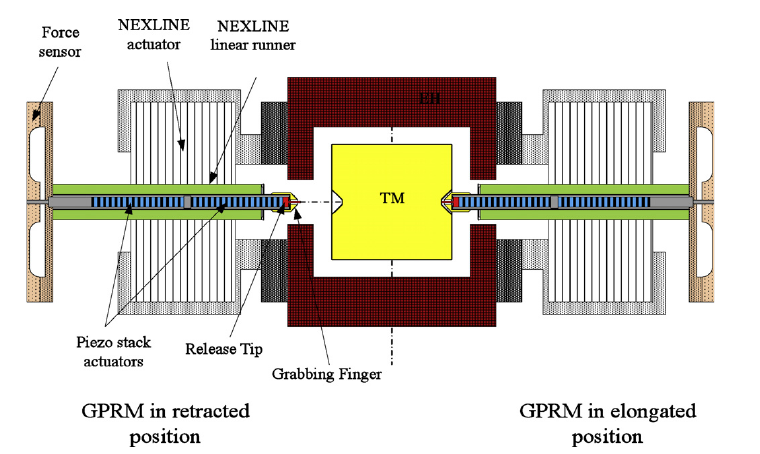
\includegraphics[scale=0.4]{gfx/GPRM}
		\end{centering}
		\caption{GPRM Mechanism}
	\end{figure}
	
	It's main parts are :
	\begin{itemize}
		\item \textit{Grabbing Finger} : holds the TM and positions it prior relase;
		\item \textit{Finger Tip} : last contact part that pons the TM in position before fast retraction for relase;
		\item \textit{Low Voltage Piezo Actuator} : used for the positioning and fast Finger Tip relase;
		\item \textit{NEXLINE actuator} : used for Grabbing Finger movement;
		\item \textit{Displacemente Sensor} : to measure the axial force acting between the mechanism contacting interface;
	\end{itemize}

	\subsubsection*{Main Task}
	The model of the injection procedure consist of three parts.\\
	The GPRM, the adhesion phenomenon and the TM motion equations.
	Two opposite GPRMs are operated simultaneously in order to hold the
	TM with the Grabbing Fingers in the center of the Electrode Housing
	(EH). From this configuration, the procedure can be considered to be symmetrical, as the two mechanism are commanded in the same way :	
	\begin{itemize}
		\item \textbf{Pre-launch and launch phase}
		\begin{enumerate}
			\item The TM is held by the Caging Mechanism (CM) at the eight corners;
		\end{enumerate}
		\item \textbf{TM Relase from CM}
		\begin{enumerate}
			\item The Grabbing Finger is in contact with the TM and the tip is fully retracted;
		\end{enumerate}
	\end{itemize}	
	The contact between the GF and the TM has to perform the following
	functions :	
	\begin{description}
		\item [{-}] Fix the TM during the release of the CM;
		\item [{-}] Center the TM in the EH;
		\item [{-}] Orient the TM with respect to the EH;
	\end{description}	
	This contact however not suitable for an undisturbated release for geodesic injection.\\ 
	The release tip must thus take over the TM pinning before
	release. 	
	\begin{itemize}
		\item \textbf{Pass Over}
		\begin{enumerate}
			\item The RT moves forward until a contact force is recorded 
			\item The GF is	retracted a small amount to compensate for the movement of the RT;
			\item The force is then reduced to the lowest acceptable level that still controls the position of the TM;
			\item TM release is performed by means of a fast contraction of the linear piezo actuator, which also commands the retraction of the tips;
			\item The TM is capture by the drag-free attitude and control system and take finally to the 					nominal center of its housing;
		\end{enumerate}
	\end{itemize}	
	We must pay attention to the fact that in presence of adhesion the
	fast retraction may cause a momentum transfer from the RTs to the TM. 

\subsection{The Physical System}
    The GPRM can be physically modeled as the lumped-element diagram reported in Figure 2 :  
    
    	\begin{figure}[H]
		\begin{centering}
			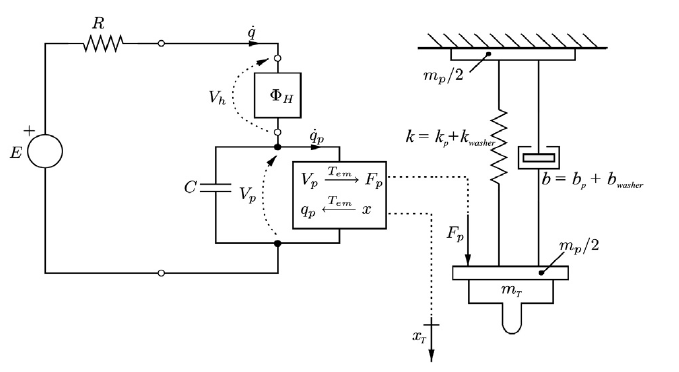
\includegraphics[scale=0.4]{gfx/phys_model}
		\end{centering}
		\caption{GPRM Physical Model}
	\end{figure}
	
		The diagram comprises the release tip mass and washer springs mounted at the extremity of the Grabbing Finger (GF) unit, and the piezo-stack actuator connected to a voltage generator through a discharge resistor R.
	
\subsection{The Mathematical Model}
    A mathematical model for the lumped-element freshly shown can be easily derived by resorting to elementary physical laws, such as the Kirchoff laws and Newton's laws, once the constitutive equations of the piezo-stack actuator are known.
    The most conventional model of a piezo-stack actuator is the one which relies on the linear constitutive equations of piezoelectric materials. \todo[inline]{inserire citazione paper} 
    Such model however is not useful for describing the dynamics of piezo-actuated positioning mechanisms because it neglects the intrinsic dynamics of the actuator. 
    A lumped parameter linear model for the piezo actuator can be obtained by manipulating the equations provided in \todo[inline]{inserire citazione paper isteresi} and by neglecting the hysteresis \todo[inline]{inserire citazione paper bortoluzzi 1} .\\
    Using the Newton and Kirchoff's laws, together with the constitutive equations of the piezoelectric transducer, and by neglecting the degree of freedom describing the suspended mass of the piezo stack\todo[inline]{inserire citazione paper bortoluzzi 2} we can obtain the equations governing the simplified model of Fig. 2 :
    
    \begin{equation}
        RC_{a}\dot{q}(t)+q(t)-T_{em}x_{T}(t)=C_{a}E(t)
    \end{equation}
    
    \begin{equation}
        m\ddot{x}_{T}(t)+ b\dot{x}_{T}(t) + \left(k+\frac{T_{em}^{2}}{C_{a}}\right) x_{T}(t) - \frac{T_{em}}{C_{a}}q(t) = 0
    \end{equation}
    
    where :
    
	\begin{itemize}
		\item $E(t)$ is the input voltage
		\item $q(t)$ is the charge accumulated on the piezo
		\item $x_{T}(t)$ is the RT position
		\item $C_{a}$ is the capacitance of the piezo stack
		\item $T_{em}$ is the piezo effect
		\item $m$ is the mass of the RT plus half of the mass of the piezo-stack
		\item $b$ is the damping coefficient
		\item $k$ is the stiffness coefficient
	\end{itemize}
	
    If the voltage $E$ and the test mass displacement $x_{T}$ are taken as the input and output variables of the system, then we can write the transfer function describing the dynamics of the GPRM as :
    
    \begin{equation}
        G(s) = \frac{X(s)}{E(s)} = \frac{b_{2}s^{2}+b_{1}s+b_{0}}{a_{3}s^{3}+a_{2}s^{2}+a_{1}s+a_{0}}
    \end{equation} 
    
    The system may be written in state space as :\\
    
    \begin{frame}
        \footnotesize
        \setlength{\arraycolsep}{1.5pt}
        \medmuskip = 0.8mu
        \thickmuskip = 0.8mu
        \small\[\scriptstyle 
            \left(\begin{array}{@{}c@{}}
            \dot{q}_{T}(t)\\
            \dot{x}_{T}(t)\\
            \ddot{x}_{T}(t)
            \end{array}\right)=\left[\begin{array}{@{}ccc@{}}
            -\frac{1}{C_{a}R} & \frac{T_{em}}{C_{a}R} & 0\\
            0 & 0 & 1\\
            \frac{T_{em}}{C_{a}m} & -\frac{k}{m}-\frac{T_{em}^{2}}{C_{a}m} & -\frac{b}{m}
            \end{array}\right]\left(\begin{array}{c}
            q(t)\\
            x_{T}(t)\\
            \dot{x}_{T}(t)
            \end{array}\right)+\left(\begin{array}{@{}ccc@{}}
            \frac{1}{R} & 0 \\
            0 & 0 \\
            0 & 1/m \\
            \end{array}\right)\left(\begin{array}{@{}cc@{}}
            E(t) & F(t) \\
            \end{array}\right)
              \]
    \end{frame}

    \begin{frame}
        \footnotesize
        \setlength{\arraycolsep}{2.5pt}
        \medmuskip = 1mu
        \thickmuskip = 1mu
        \small\[\scriptstyle 
            {y}(t) = 
            \left[\begin{array}{@{}ccc@{}}
            0 & 1 & 0\\
            \end{array}\right]\left(\begin{array}{@{}c@{}}
            q(t)\\
            x_{T}(t)\\
            \dot{x}_{T}(t)
            \end{array}\right)
                \]
    \end{frame}\\   
    
    where the elements $A_{1,1}$, $A_{1,2}$, $A_{3,1}$, $A_{3,2}$, $A_{3,3}$, $B_{1}$ are unknown and will be estimated in identification (Sec 3.1).
    
    \subsubsection{Test mass model}  
    TM is easily modeled as a rigid body in free motion, Newton's equations describe linear displacement dynamics
    
    \begin{align*}
        M\uline{\ddot{x}}_{TM} &= \uline{F}
        %M\ddot{y}_{TM} &= F_y\\
        %M\ddot{z}_{TM} &= F_z
    \end{align*} 
    
    while Euler's equations
    
    \begin{align*}
        \uuline{J}\uline{\dot{\omega}}+\uuline{J}\uline{\omega}\times\uline{\omega}=\uline{M}
    \end{align*}
    
    can be simplified in this case since inertia moment I is the same for each of the 3 principal axes ($J_{i,j} =I \delta_{i,j}$) and describe angular dynamics : 
    
    \begin{align*}
        I\uline{\dot{\omega}}&=\uline{M}
    \end{align*}
    
    To complete the model, a set of kinematic equations for angular motion shall be considered :
    
    \begin{equation*}
        \uuline{\dot{A}}+\big[\uuline{\omega}^{\wedge}\big]\uuline{A} =0
    \end{equation*}
    
    This last equation can be substituted by different models i.e. Euler Angles kinematic equations that can be more suitable. A simplified model have been derived considering system simmetry. Force components on y and z axes arise due to TM rotation. Angular velocity is expected to be of the order of few $\mu rad/s$, the contact between TM and RTs lasts much less than $1 ms$, as a result rotation angle is a fraction of $nrad$ and is neglected. Rotation arises for a modeled misalignment on y-axis only. So the linear dynamics as well as the rotational ones occur on one axis only. Therefore the system is widely simplified:
    
    \begin{empheq}[left = \empheqlbrace]{align}
        &M\ddot{x_T}=F\\ 	
        &I\dot{\omega}=M\\ 
        &\dot{\theta}=\omega
    \end{empheq}
    
    \subsubsection{Adhesion force model}
        \begin{table*}
        \setlength{\tabcolsep}{0.35 cm}
        \renewcommand{\arraystretch}{1.2}
        \begin{tabular}{c| c c|c c|c c }
        \textbf{Coefficient} & \multicolumn{2}{c|}{\textbf{set 1}}&\multicolumn{2}{c|}{\textbf{set 2}}& \multicolumn{2}{c}{\textbf{set 3}}\\
            &mean value & std.dev. & mean value & std.dev. &mean value & std.dev. \\ \hline
            $X_1$& $0.50$&$2.59 \times 10^{-2}$ & $ 0.357$ & $ 7.30 \times 10^{-2}$ &$0.457$ & $3.58 \times 10^{-2}$\\
            $X_2$ & $2.89$ & $2.75 \times 10^{-1}$ & $1.32$ & $1.59\times 10^{-1}$ & $1.73$ & $1.22\times 10^{-1}$\\
            $X_3$ & $2.36$ & $4.76\times 10^{-2}$ & $2.07$ & $2.14 \times 10^{-1}$ & $1.27$ & $2.98 \times 10^{-1}$\\
        \end{tabular}
            \caption{adhesion force fitting results}
        \end{table*}
        
    The following description of the adhesion force competes the model. A dynamic model for tip actuation and TM motion has been derived and it includes a parametric representation of force acting on tip and which is an input of the system. The description of adhesion force starts with experimental data shown in Fig. 3, that presents several experimental measurments for 3 different sets. 
    
    \begin{figure}[t]
        \begin{centering}
			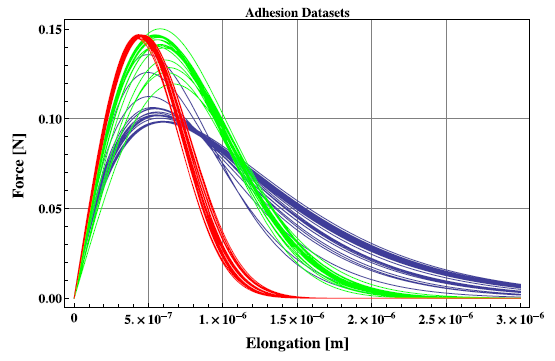
\includegraphics[scale=0.6]{gfx/adh_data}
		\end{centering}
            \caption{Adhesion force experimental data (from Bortoluzzi et al. 2012)}
        \end{figure}
        
    Following the procedure adopted by Bortoluzzi  \todo[inline]{inserire citazione paper bortoluzzi 2}, once experimental data are sampled from Fig.3, they are fitted into exponential model:\\
    
    \begin{equation*}
        F_{ad}(\Delta l)=X_1\Delta l e^{X_2\Delta l^{X_3}} \\
    \end{equation*}
    The MATLAB \textbf{lsqcurvefitting} routine is then used to perform a least square minimization fitting of the experimental data. Resulting $X_1,X_2,X_3$ coefficients and their standard deviations are listed in table 2.
    
    \begin{figure}[t]
		\begin{centering}
			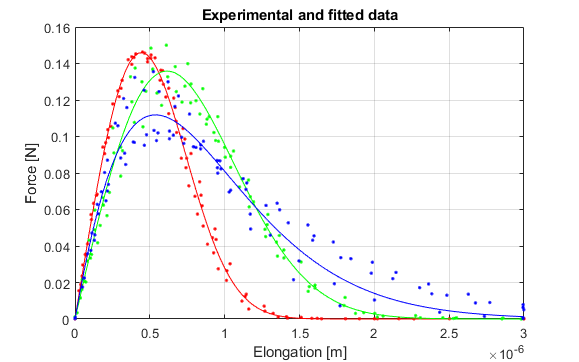
\includegraphics[scale=0.6]{gfx/adh_all}
		\end{centering}
            \caption{Adhesion force sampled data and fittings}
    \end{figure}
    
    \subsubsection{Contact force model and preload}
    
\section{Simulation}
\begin{table*}[t]
    \setlength{\tabcolsep}{0.5 cm}
    \renewcommand{\arraystretch}{1.2}
    \begin{tabular}{|c |c c c c c|}\hline
    parameter & guessed value & lower bound & upper bound & identified value & unit \\ \hline
    $C_a$ & $4.8\times 10^{-7}$ & 0 & $10^{-6}$ & $3.936 \times 10^{-7}$ & F \\
    $T_{em}$ & $1.5$ & 0 & - & $1.51$ & $\sqrt{\nicefrac{FN}{m}}$ \\
    R & 400 & 100 & 800 &417 & $\Omega$\\
    m & $10^{-3}$ & $10^{-4}$ &0.014 & $10^{-4} $ & kg\\
    b & 150 & 100 & - & 100 & $\nicefrac{Ns}{m}$ \\
    k & $1.5 \times 10^7$ & 0 & - & $1.5 \times 10^7$ & $\nicefrac{m}{s}$\\
    $V_0$ & 0 & -0.05 & 0.05 & $3 \times 10^{-3}$ & $\nicefrac{m}{s}$ \\ \hline
    \end{tabular}
        \caption{Identification inputs and results}
\end{table*}

    \subsection{Identification}
        Identification makes use of experimental data to estimate unknown parameters of the model. Experimental data are extrapolated from \todo[inline]{inserire citazione paper bortoluzzi 2} and are resampled with a 1MHz frequency to be consistent with the cited paper data. 
        The parameters to be identified are the six physical constants that appear nonlinearly in RT linear system, the $V_0$ initial velocity of the RT parametrized as: \\
    \\
    \begin{centering}
    $
        \begin{pmatrix}
            q(0) \\
            x_T(0) \\
            \dot{x}_T(0)
        \end{pmatrix}
    =
    \begin{pmatrix}
        0 \\
        0 \\
        V_0
    \end{pmatrix}
    $
    \end{centering}
    \\
    \\
    Therefore, the vector of parameters to be estimeted is defined as :\\
    \\
    \begin{centering}
        $\textbf{p} = 
        \begin{bmatrix}
            C_a \\
            T_{em} \\
            R \\
            m \\
            b \\
            k \\
            V_0
    \end{bmatrix}
    $
    \end{centering}
    \\
    \\
    Identification consists in minimaze the variance of the residual between measured and modeled responce:\\
    \\
    $ \textbf{p}=argmin(\psi_N(\textbf{p}))$\\
    \\
    with penalty function $\psi_N$ defined as:\\
    \\
    $\psi_N(\textbf{p})=\frac{1}{N}\sum\limits_{i=1}^N(y_N(t_i)-y(t_i|\textbf{p}))^2$\\
    where $y_N$ is the experimental responce and $y(t_i|\textbf{p})$ is the modeled responce with parameter set \textbf{p}.\\
    Identification is performed with MATLAB \textbf{pem} command using the Levenberg-Marquardt search method. Due to non linearity of the problem many local minima can be found and  in order to have the routine converging to a solution with physical meaning appropriate initial guess for \textbf{p} must be set, as well as suitable constrains (i.e. a lower bound to avoid physical parameters converging to a negative value). \\
    
    \begin{figure}
            \begin{centering}
                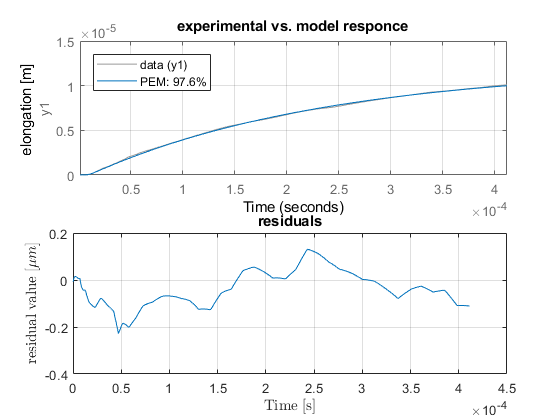
\includegraphics[scale=0.6]{gfx/Identification_results}
            \end{centering}
                \caption{Comparison between modeled and experimental responce}
    \end{figure}
    
    Estimated parameters are reported in Table 3. Figure 4 shows the comparison between experimental and identified model responce. Residuals are small, always <1\% of max. tip retraction, their RMS is $x_{T,rms}=84 nm$.\\

    \subsection{Monte Carlo simulation}
    In Sec. 3.1 nominal values of tip actuation mechanism parameters have been estimated. However some deviation of the actual mechanism from the nominal one may occur. The simulation is performed through a Monte-Carlo approach: the simulation of the release phase is repeated many times changing the model of the mechanism. The results of this procedure will be the \textit{Probability Density Function} of some relevant quantities.
    
    \subsubsection{Parameters uncertainty}
    Two approaches are followed to include parameters uncertainty into the simulation.\\
    The first one consists in letting each parameter assume in each simulation a random value with a suitable probability distribution. A covariance matrix is computed with the formula :\\
    
    \begin{equation*}
        \Sigma_p=\big(J^T\Sigma_x^{-1}J\big)^{-1}
    \end{equation*}
    
    where J is the jacobian. Being $x_i$ the retraction at i-th time step and $p_j$ the j-th parameter, J is defined as :\\
    
    \begin{equation*}
        J_{ij}=\frac{\partial x_i}{\partial p_j}\\
    \end{equation*}
    
    Jacobian is estimated by performing simulations of the nominal mechanism and of the mechanism with a parameter shifted from nominal one with an high order integrator (\textit{ode113} was adopted for this purpose) and then comparing the responces. Being $res_i$ the residual at i-th time step, $\Sigma_x$ is built as :
    
    \begin{equation*}
        \Sigma_x = 
        \begin{pmatrix}
            res_1^2& 0 & \cdots & 0\\
            0 & res_2^2 & \cdots & 0\\
            \vdots & \vdots & \ddots & \vdots \\
            0 & 0 & \cdots & res_N^2
        \end{pmatrix}
    \end{equation*}\\
    
    A final form for covariance matrix accounts both for identification and \textit{a priori} uncertainties, here quantified as standard deviation $\sigma_0=0.3\times p$ for each parameter. Being $\Sigma_{p,0}^-1$ the a priori covariance matrix, covariance matrix is then defined as :
    
    \begin{equation*}
        \Sigma_p=\big(\Sigma_{p,0}^{-1}+J^T\Sigma_x^{-1}J\big)^{-1}
    \end{equation*}\\
    
    Eventually no correlation is assumed, so off-diagonal elements are ignored.\\
    The main issue with this approach is the inversion of left hand side of equation \todo[inline]{put previous equation number}, which may yield inaccurate results. In this case, although high conditioning number, results appear consistent. The second approach consists in altering the tip retraction dynamics by a fotce F(t) applied on the tip which generates a displacement with same \textit{Power Spectral Density} (PSD) as the residual. The procedure is depicted in the main steps as follows :
    
    \begin{align*}
        res& & &\text{residuals}\\ 
        &\Downarrow \\
        C_{res,res}&=res \ast res & &\text{auto correlation}\\ 
        &\Downarrow \\ 
        PSD_{2-sided}&=fft(C_{res,res}) & &\text{Fourier transform}\\
        &\Downarrow \\
        PSD\times n_w(j\omega)&=res_{rand} &&\text{white noise filtering}\\
        &\Downarrow \\
        F_{rand}(j\omega)&=\frac{res_{rand}}{H(j\omega)} &&\text{force in Fourier domain}\\
        &\Downarrow\\
        F_{rand}(t)&=ifft(F_{rand}(j\omega)) &&\text{force in time domain}
    \end{align*}
    
    Residual auto-correletion is transformed into Fourier domain to get the PSD, shown in \todo[inline]{inserire numero figura PSD}. Then a white noise, in frequency domain too, is filtered through the PSD. The filtered noise is a simulated random displacement, in order to use it in the simulation, it must pass through the \textit{Frequency Responce Function} (FRF), here called $H(j\omega)$, whose expression is stated below :
    
    \begin{equation*}
        H(j\omega)=\frac{X(j\omega)}{F(j\omega)}=\frac{b(j\omega)+1}{a_3(j\omega)^3+a_2(j\omega)^2++a_1(j\omega)+a_0}\\
    \end{equation*}
    
    where:
    
    \begin{empheq}[left = \empheqlbrace]{align*}
        b&=R C_a\\
        a_0&=k\\
        a_1&=b+RT_{em}^2+RC_ak\\
        a_2&=m+RbC_a\\
        a_3&=RC_am
    \end{empheq}
    
    The resut is the random force to be applied on the tip in Fourier domain. \todo[inline]{inserire numero figura quantità in dominio di Fourier} shows FRF, displacement and force in frequency domain.Eventually the force is turned in time domain using inverse Fourier transform (\todo[inline]{inserire numero figura forza}).
    
    \begin{figure}[H]
        \begin{centering}
			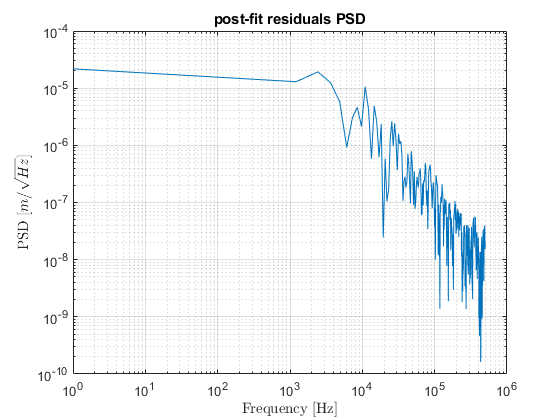
\includegraphics[scale=0.6]{gfx/PSD}
		\end{centering}
            \caption{residuals 1-sided PSD in logaritmic plot}
    \end{figure}

    This method has two main numerical criticalities :
    
    \begin{enumerate}   
        \item The procedure described would be mathematically exact if signals to process where infinite in               extension. The fact that the bandwidth is limited to [$-5\times10^5- 5\times10^5$]Hz (1MHz sampling frequency) is not critical because the low-pass fiter like PSD behaviour is such that high frequences would be anyway filtered away. On the other hand the residual is finite and this makes the auto-convolution inaccurate.
        \item Displacement noise is divided by $H(j\omega)$, which is an FRF with a zero and may lead to    numerical issues.
    \end{enumerate}

    \begin{figure}[H]
		\begin{centering}
			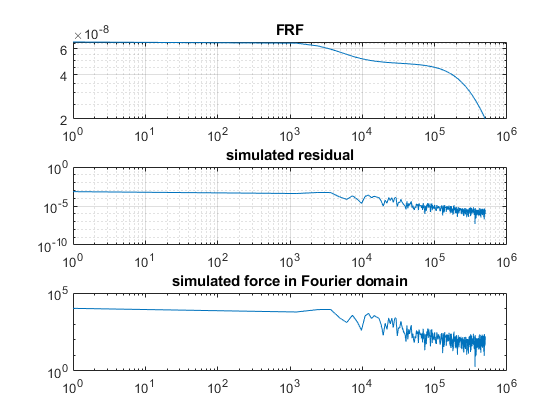
\includegraphics[scale=0.6]{gfx/F_domain}
		\end{centering}
            \caption{FRF and examples of residual and force in Fourier domain}
    \end{figure}
    \begin{figure}[H]
		\begin{centering}
			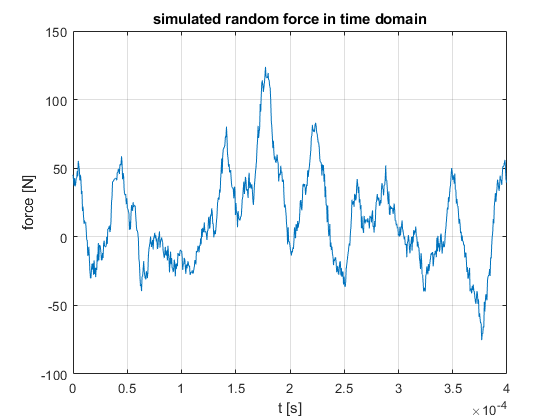
\includegraphics[scale=0.6]{gfx/Force}
		\end{centering}
            \caption{An example of random force to be applied to the tip obtained through the described procedure}
    \end{figure}

% Citazioni
    citazione \cite{latexcompanion}
    \begin{thebibliography}{9}
        \bibitem{latexcompanion} 
            Michel Goossens, Frank Mittelbach, and Alexander Samarin. 
            \textit{The \LaTeX\ Companion}. 
            Addison-Wesley, Reading, Massachusetts, 1993.
        \bibitem{einstein} 
            Albert Einstein. 
        \textit{Zur Elektrodynamik bewegter K{\"o}rper}. (German) 
    [\textit{On the electrodynamics of moving bodies}]. 
    \bibitem{knuthwebsite} 
        Knuth: Computers and Typesetting,
    \\\texttt{http://www-cs-faculty.stanford.edu/\~{}uno/abcde.html}
    \end{thebibliography}
\end{document}
